%%%%%%%%%%%%%%%%%%%%%%%%%%%%%%%%%%%%%%%%%
% Beamer Presentation
% LaTeX Template
% Version 1.0 (10/11/12)
%
% This template has been downloaded from:
% http://www.LaTeXTemplates.com
%
% License:
% CC BY-NC-SA 3.0 (http://creativecommons.org/licenses/by-nc-sa/3.0/)
%
%%%%%%%%%%%%%%%%%%%%%%%%%%%%%%%%%%%%%%%%%

%----------------------------------------------------------------------------------------
%	PACKAGES AND THEMES
%----------------------------------------------------------------------------------------

\documentclass[t]{beamer}

\mode<presentation> {

% The Beamer class comes with a number of default slide themes
% which change the colors and layouts of slides. Below this is a list
% of all the themes, uncomment each in turn to see what they look like.

%\usetheme{default}
%\usetheme{AnnArbor}
%\usetheme{Antibes}
%\usetheme{Bergen}
%\usetheme{Berkeley}
%\usetheme{Berlin}
%\usetheme{Boadilla}
%\usetheme{CambridgeUS}
%\usetheme{Copenhagen}
%\usetheme{Darmstadt}
%\usetheme{Dresden}
%\usetheme{Frankfurt}
%\usetheme{Goettingen}
%\usetheme{Hannover}
%\usetheme{Ilmenau}
%\usetheme{JuanLesPins}
%\usetheme{Luebeck}
\usetheme{Madrid}
%\usetheme{Malmoe}
%\usetheme{Marburg}
%\usetheme{Montpellier}
%\usetheme{PaloAlto}
%\usetheme{Pittsburgh}
%\usetheme{Rochester}
%\usetheme{Singapore}
%\usetheme{Szeged}
%\usetheme{Warsaw}

% As well as themes, the Beamer class has a number of color themes
% for any slide theme. Uncomment each of these in turn to see how it
% changes the colors of your current slide theme.

%\usecolortheme{albatross}
%\usecolortheme{beaver}
%\usecolortheme{beetle}
%\usecolortheme{crane}
%\usecolortheme{dolphin}
%\usecolortheme{dove}
%\usecolortheme{fly}
%\usecolortheme{lily}
%\usecolortheme{orchid}
%\usecolortheme{rose}
%\usecolortheme{seagull}
%\usecolortheme{seahorse}
%\usecolortheme{whale}
%\usecolortheme{wolverine}

%\setbeamertemplate{footline} % To remove the footer line in all slides uncomment this line
%\setbeamertemplate{footline}[page number] % To replace the footer line in all slides with a simple slide count uncomment this line

%\setbeamertemplate{navigation symbols}{} % To remove the navigation symbols from the bottom of all slides uncomment this line
}

\usepackage{graphicx} % Allows including images
\usepackage{booktabs} % Allows the use of \toprule, \midrule and \bottomrule in tables
\usepackage{fancyvrb} % Tabs in verbatim
%----------------------------------------------------------------------------------------
%	TITLE PAGE
%----------------------------------------------------------------------------------------

\title[uC102]{uC102: Embedded Communication Protocols / ADC} % The short title appears at the bottom of every slide, the full title is only on the title page

\author{Josh Johnson} % Your name
\institute[] % Your institution as it will appear on the bottom of every slide, may be shorthand to save space
{ \\ % Your institution for the title page
\medskip
\textit{} % Your email address
}
\date{8/7/2019} % Date, can be changed to a custom date

\begin{document}

\begin{frame}
\titlepage % Print the title page as the first slide
\end{frame}

%----------------------------------------------------------------------------------------
%	PRESENTATION SLIDES
%----------------------------------------------------------------------------------------

\begin{frame}
\frametitle{Overview}
\begin{itemize}
\item Embedded communication requirements
\item UART - Universal Asynchronous Receiver Transmitter
\item Tangent: Debugging
\item SPI - Serial Peripheral Interface
\item Tangent: Manchester Encoding
\item I2C - Inter-Integrated Circuit 
\item JTAG	- Joint Test Action Group
\item ADC - Analog to Digital Converter
	

\end{itemize}
\vspace{20mm}
Project Files: \url{github.com/joshajohnson/CBRhardware}\\
\end{frame}

%----------------------------------------------------------------------------------------

\begin{frame}[t]
\frametitle{Embedded communication requirements}
\begin{itemize}
	\item Typically an embedded processor communicating with peripherals.
	\item Typically single master, multiple slave system.
	\item Multi master (eg CAN) does exist, out of scope for today.
	\item UART/SPI/I2C is probably over 99\% of embedded communications.
\end{itemize}
\vspace{5mm}
\textbf{Common peripherals}
\begin{itemize}
	\item Inertial Measurement Unit (Gyroscope, Accelerometer)
	\item SPI Flash Chip / EEPROM
	\item RF Transmitter
	\item Display
	\item Addressable LEDs
\end{itemize}

\end{frame}

%----------------------------------------------------------------------------------------

\begin{frame}[t]
\frametitle{Where on the OSI Model?}
We are dealing with layer one and two of the OSI model. 
\begin{figure}
	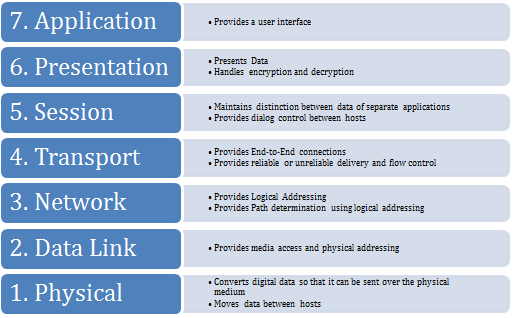
\includegraphics[width=0.8\linewidth]{osiModel.png}
\end{figure}

\end{frame}

%----------------------------------------------------------------------------------------

\begin{frame}[t]
\frametitle{What Physical Medium?}
\begin{figure}
	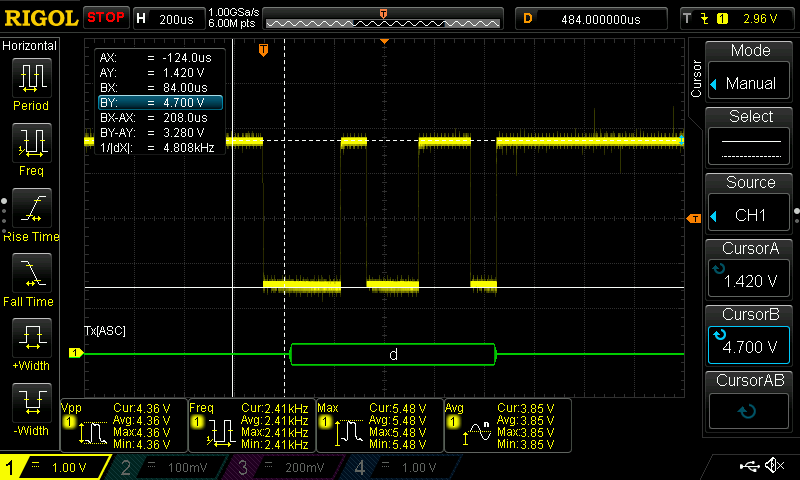
\includegraphics[width=0.9\linewidth]{badSerial.png}
\end{figure}
Oscilloscope trace of a (bad) 5V CMOS signal. 
\end{frame}

%----------------------------------------------------------------------------------------

\begin{frame}[t]
\frametitle{What Physical Medium?}
Digital data over wires, looking at voltage with respect to time. \\
Dark colour is output voltage from chip, light input voltage to chip.
\begin{figure}
	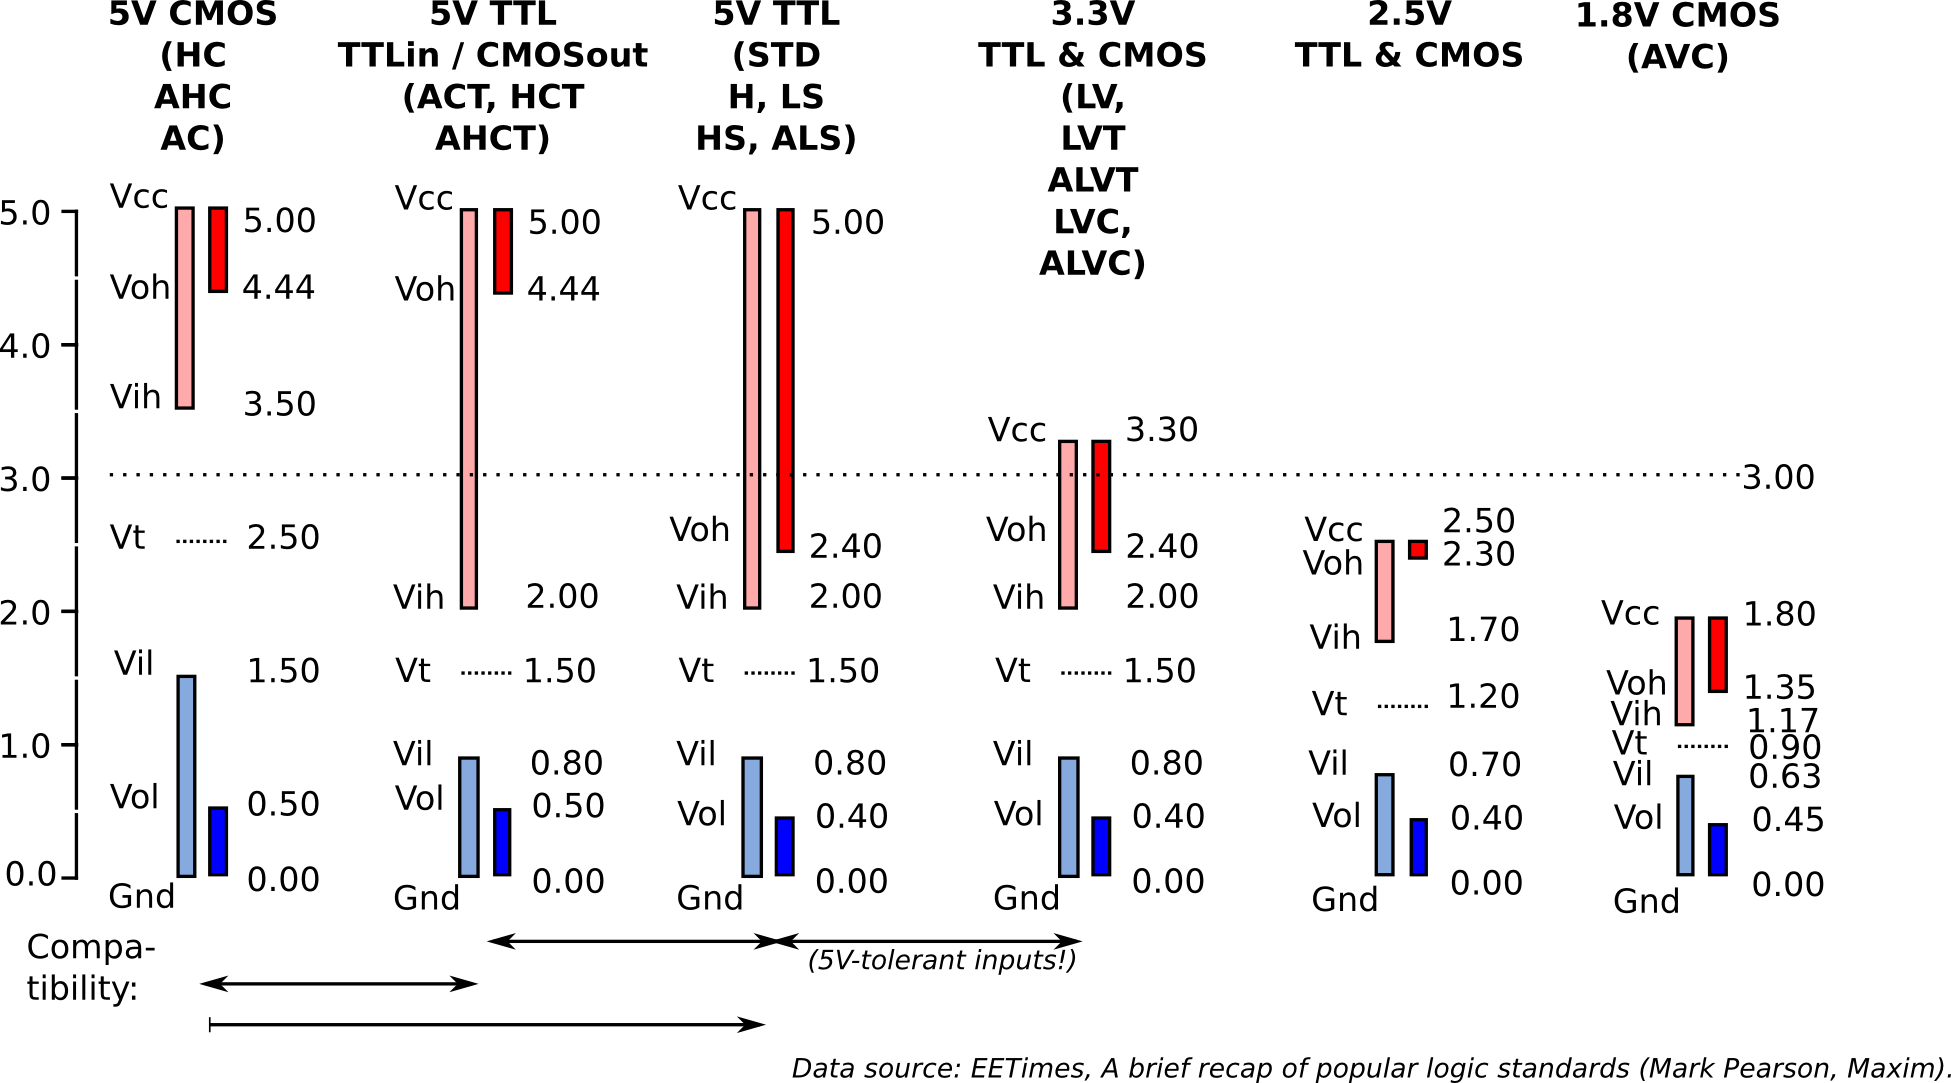
\includegraphics[width=0.8\linewidth]{logicLevels.png}
\end{figure}

\end{frame}

%----------------------------------------------------------------------------------------

\begin{frame}[t]
\frametitle{Universal Asynchronous Receiver Transmitter}
\begin{itemize}
	\item \textbf{Asynchronous: }not coordinated in time, i.e. no shared clock.\\
	\item Two wires, TX and RX.\\
	\item Device 1 TX connects to Device 2 RX, and vice versa. 
	\item Accurate clock required for devices to stay in sync.
	\item Both devices must agree on frame for successful communication.
	\begin{itemize}
		\item Bits per second (baud rate).
		\item Bits per transfer.
		\item Number of stop bits.
		\item Parity bit (even/odd/none).
		\item LSB / MSB first.
		\item Inverted. 
	\end{itemize}
	\item 9600 baud, 8N1 is the most common (8 bits per transfer, no parity, 1 stop bit). 
\end{itemize}

\end{frame}

%----------------------------------------------------------------------------------------

\begin{frame}[t]
\frametitle{UART}
\begin{figure}
	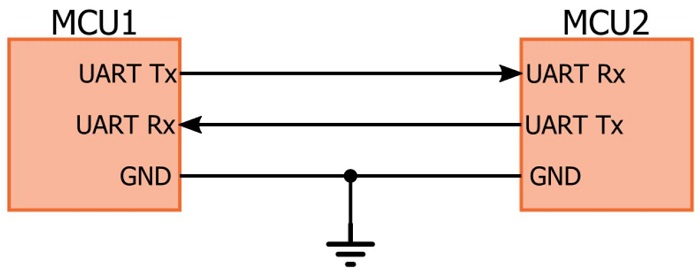
\includegraphics[width=0.5\linewidth]{uartConfig.jpg}
\end{figure}
\begin{center}
	Typical UART connection.
\end{center}
\begin{figure}
	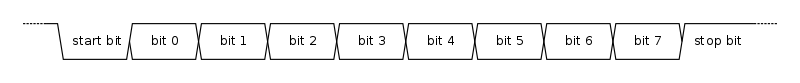
\includegraphics[width=0.9\linewidth]{uartFrame.png}
\end{figure}
\begin{center}
	Typical UART data frame.
\end{center}

\vspace{3mm}
Regarding the need for accurate clocks:\\
Ben Eater: https://youtu.be/eq5YpKHXJDM?t=1590 (26:30 in)
\end{frame}

%----------------------------------------------------------------------------------------

\begin{frame}[t]
\frametitle{How to Debug}
\begin{itemize}
	\item Oscilloscope
	\item Logic Analyser
	\item Try known good HW / SW
\end{itemize}
\begin{figure}
	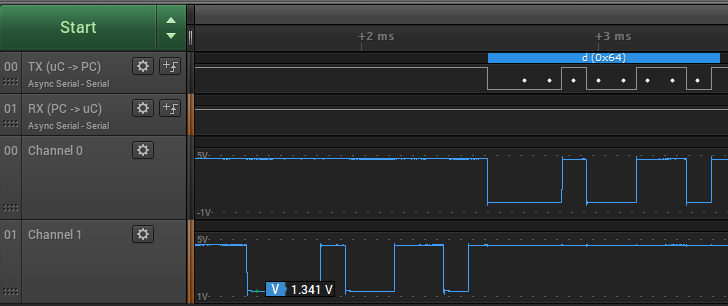
\includegraphics[width=0.9\linewidth]{serialNotWorking.png}
\end{figure}
Logic capture of the UART comms with my PC.
\end{frame}

%----------------------------------------------------------------------------------------

\begin{frame}[t]
\frametitle{How to Debug}
\begin{figure}
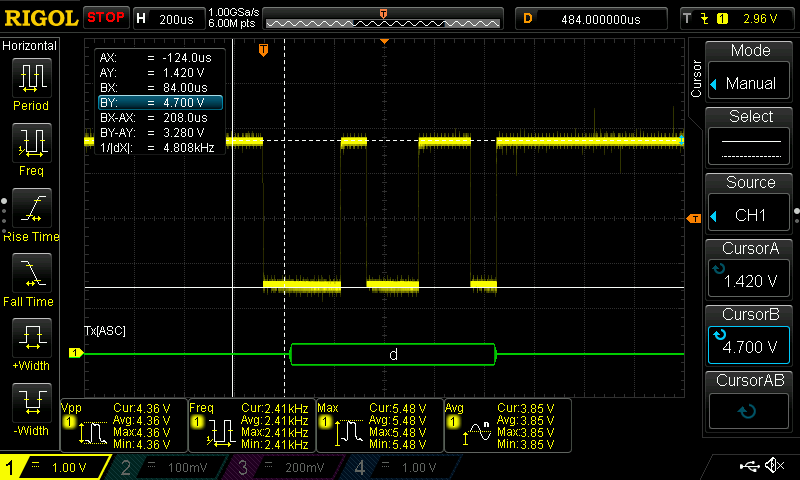
\includegraphics[width=0.9\linewidth]{badSerial.png}
\end{figure}
Note the low voltage of 1.4V, not the 0 we expected. 
\end{frame}

%----------------------------------------------------------------------------------------

\begin{frame}[t]
\frametitle{Serial Peripheral Interface}
\begin{itemize}
	\item Synchronous, full duplex master-slave-based interface.
	\item 4 wires, SCLK, MOSI, MISO, nCS.
	\item Data is synchronised on rising or falling clock edge.
	\item Single master, data simultaneously transmitted in and out.
	\begin{itemize}
		\item Clock Polarity (CPOL)
		\item Clock Phase (CPHA)
		\item MSB vs LSB first
	\end{itemize}
	\item To determine, check the timing diagrams for your specific chip, as we will see tonight SPI has many implementations.
\end{itemize}

\end{frame}

%----------------------------------------------------------------------------------------

\begin{frame}[t]
\frametitle{SPI}

\begin{figure}
	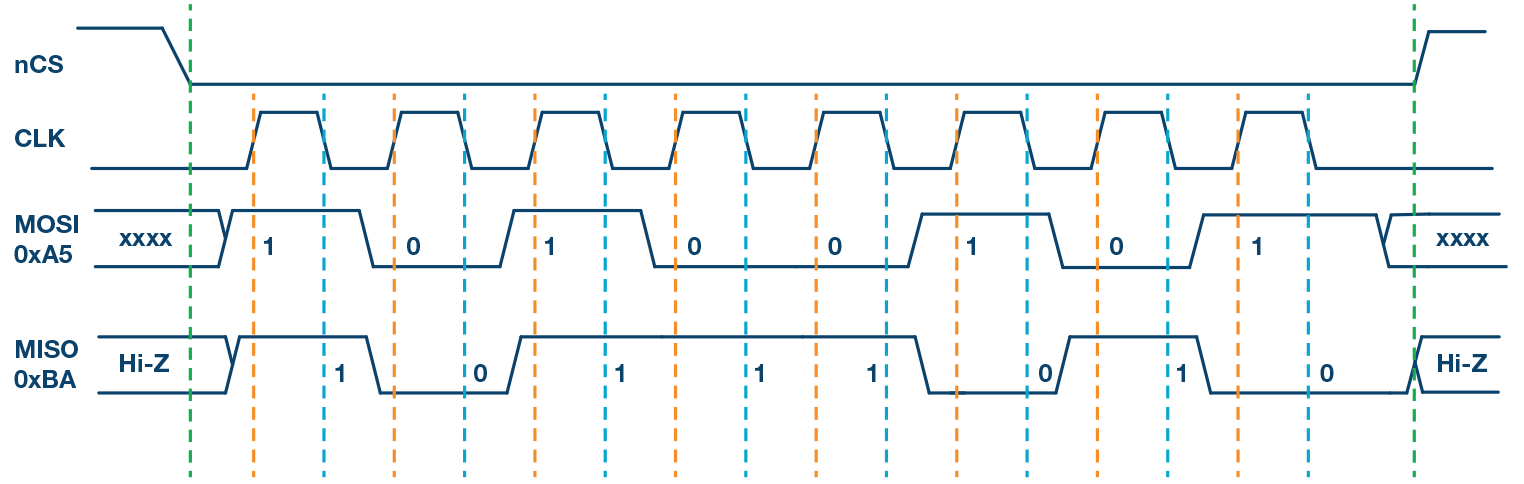
\includegraphics[width=0.7\linewidth]{spiMode0.png}
\end{figure}
SPI Mode 0, CPOL = 0, CPHA = 0: CLK idle state = low, data sampled on rising edge and shifted on falling edge.
\begin{figure}
	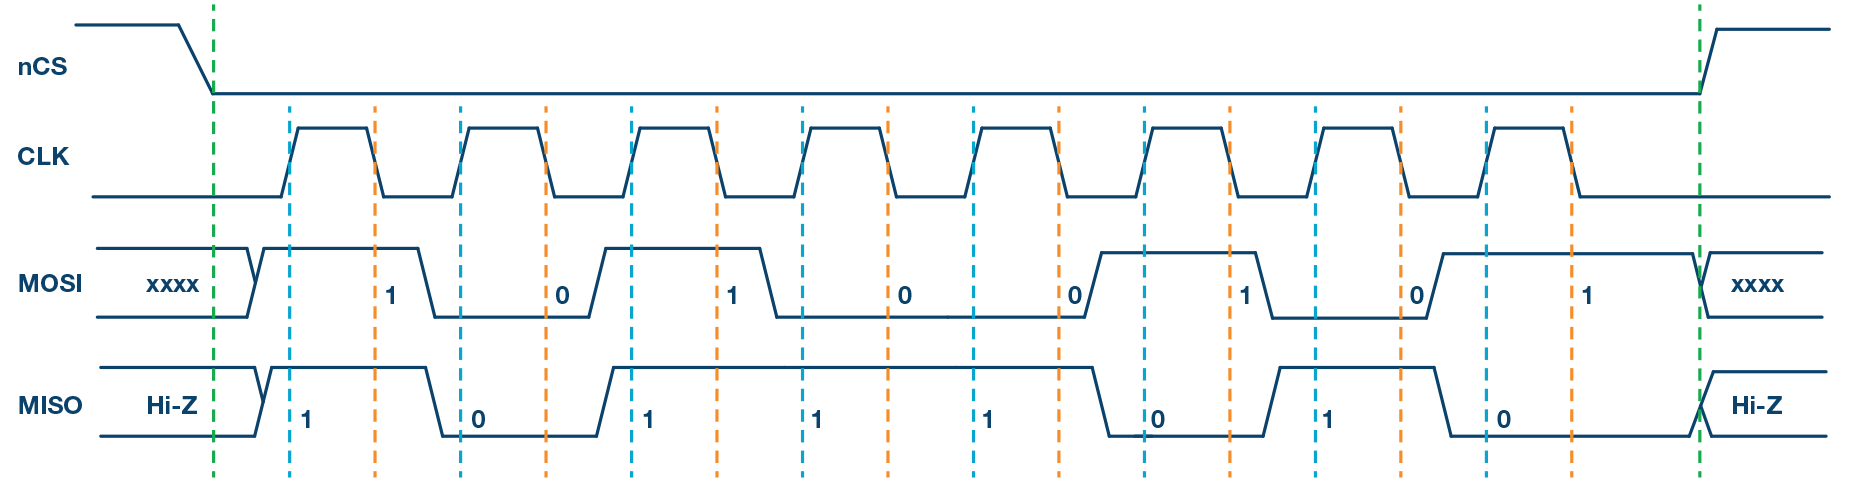
\includegraphics[width=0.7\linewidth]{spiMode1.png}
\end{figure}
SPI Mode 1, CPOL = 0, CPHA = 1: CLK idle state = low, data sampled on the falling edge and shifted on the rising edge.
\end{frame}

%----------------------------------------------------------------------------------------

\begin{frame}[t]
\frametitle{SPI}
Multiple devices can be connected to same SPI bus if they use the same communication settings. 
\begin{figure}
	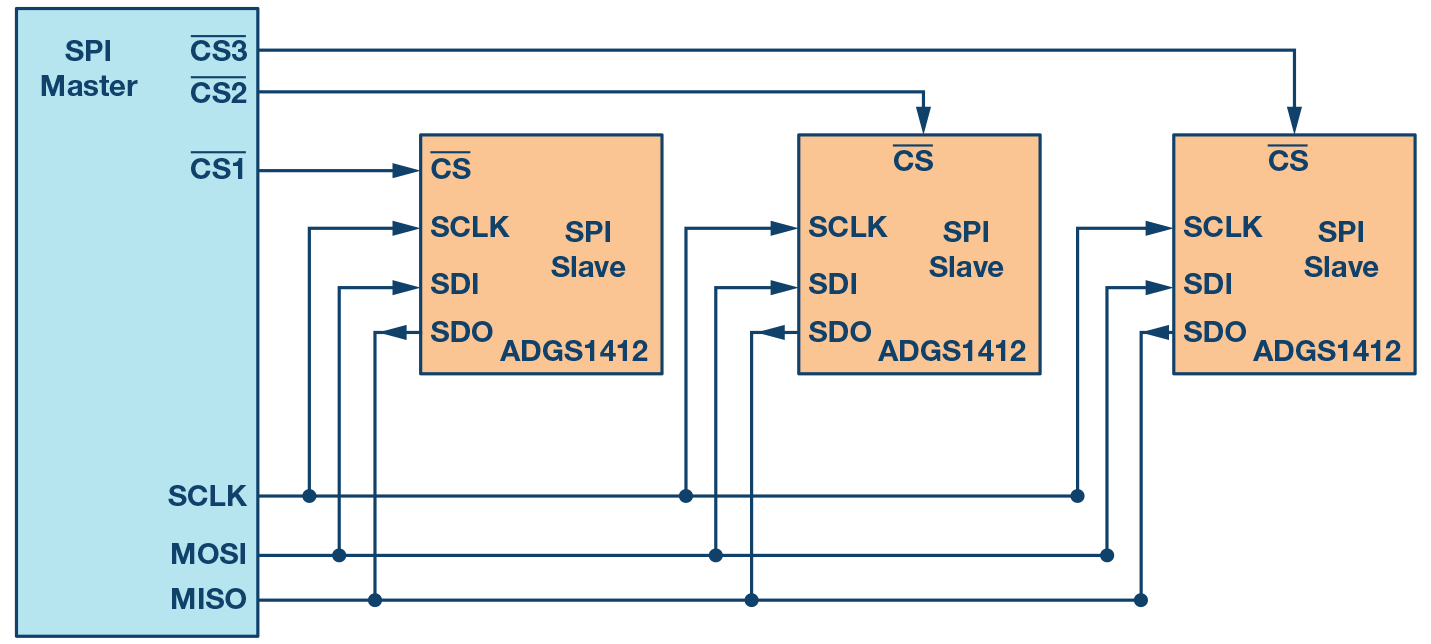
\includegraphics[width=0.9\linewidth]{spiMultiSlave.png}
\end{figure}
Regular multislave SPI configuration.
\end{frame}

%----------------------------------------------------------------------------------------

\begin{frame}[t]
\frametitle{SPI}
Datasheet Time!
\begin{itemize}
	\item APA102 addressable LEDs
	\item MAX2871 PLL 
\end{itemize}

\end{frame}

%----------------------------------------------------------------------------------------

\begin{frame}[t]
\frametitle{Tangent: Manchester Encoding}
Manchester encoding integrates a clock into the transmitted signal, however halves the bandwidth. \\
\begin{figure}
	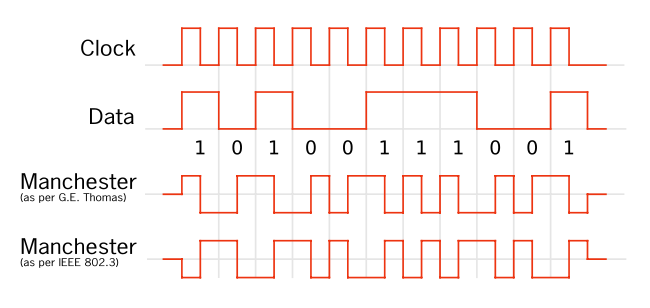
\includegraphics[width=0.9\linewidth]{manchester.png}
\end{figure}
Used in car keyfobs, 10Base-T ethernet (IEEE 802.3), amongst others. 
\end{frame}

%----------------------------------------------------------------------------------------

\begin{frame}[t]
\frametitle{Tangent: Manchester Encoding}
\begin{columns}
	\column{.49\textwidth}
		\begin{figure}
			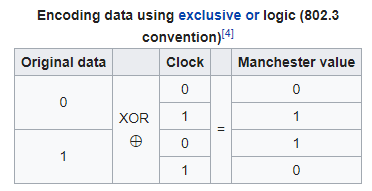
\includegraphics[width=\linewidth]{manchesterCalculation.png}
		\end{figure}
		Calculating the Manchester encoded signal.
	
	\column{.5\textwidth}
		\begin{figure}
			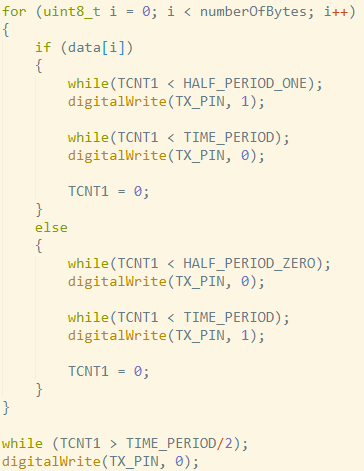
\includegraphics[width=0.7\linewidth]{manchesterArduino.png}
		\end{figure}
		Arduino implementation of Manchester encoding 
	
\end{columns}
\end{frame}

%----------------------------------------------------------------------------------------

\begin{frame}[t]
\frametitle{Joint Test Action Group}
\begin{itemize}
	\item 4 wires, TCK, TDI, TDO, TMS.
	\item Serial connection similar to SPI, however devices are daisy chained. 
	\item Originally designed to test complicated (BGA, high density) boards.
	\item Later used to program and debug ICs.
	\item SWD uses a reduced pin count version of JTAG with two wires (SWDIO, SWCLK). 
\end{itemize}
\begin{figure}
	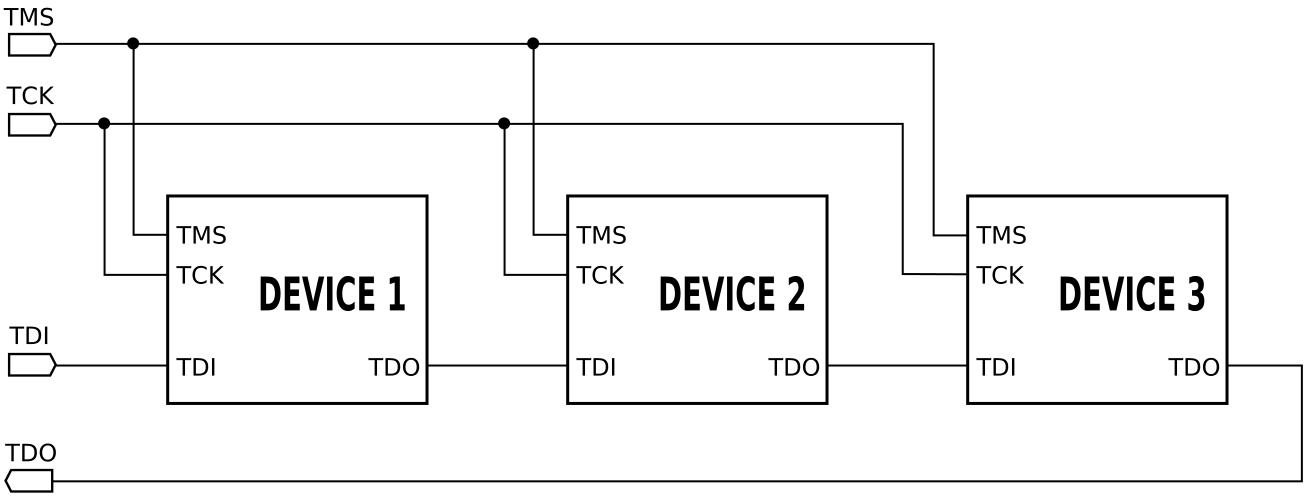
\includegraphics[width=0.7\linewidth]{jtagChain.png}
\end{figure}

\end{frame}

%----------------------------------------------------------------------------------------

\begin{frame}[t]
\frametitle{JTAG}
\begin{figure}
	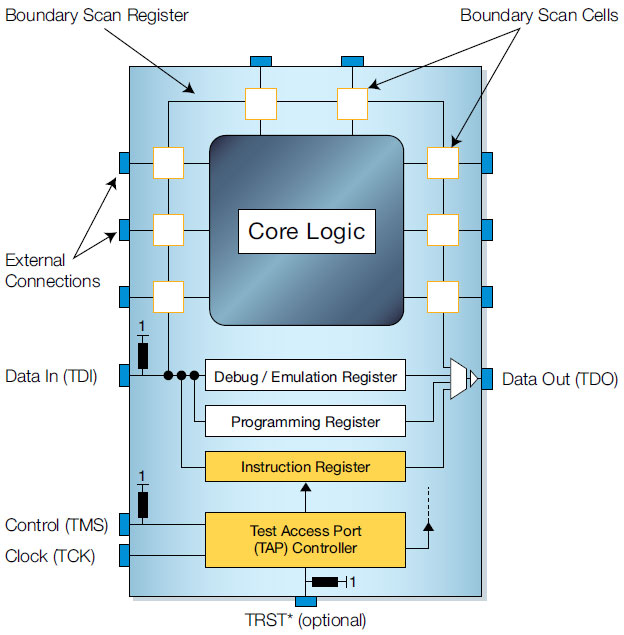
\includegraphics[width=0.5\linewidth]{jtagInternals.jpg}
\end{figure}
Internal architecture of an IC supporting JTAG.
\end{frame}

%----------------------------------------------------------------------------------------

\begin{frame}[t]
\frametitle{JTAG}

\begin{columns}
	\column{.7\textwidth}
	\textbf{Boundary Scan}
	\begin{itemize}
		\item Automated testing of all connections on board.
		\item Utilises BSDL (Boundary Scan Description Language) file for each component, which defines pin types. 
		\item Can test components on single board, or connect multiple boards together to scan complicated system. 
		\item Looks for stuck high, stuck low, pins tied together, not connected. 
		\item Requires external software and programmer to configure. 
		\item Used in production testing to check for bad connections.
	\end{itemize}
	
	\column{.29\textwidth}
	\begin{figure}
		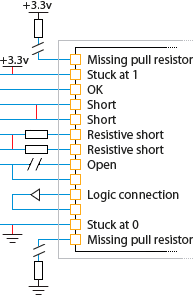
\includegraphics[width=\linewidth]{boundaryScanFaults.png}
	\end{figure}
\end{columns}

\end{frame}

%----------------------------------------------------------------------------------------

\begin{frame}[t]
\frametitle{JTAG}
\textbf{Programming / Debugging}
\begin{itemize}
	\item Can be used to program flash / configure FPGA / etc.
	\item Low level connections into IC allow for register level debug.
	\item Manufactures implement their own commands which can be called by JTAG to set breakpoints, read registers etc.
	\item Due to use in production, JTAG often left exposed on PCB with no protections. 
	\item This allows user to control JTAG device if they have physical access. 
	\item Devices (e.g. ATmega) may have JTAG, but may not be used. ICSP (In Circuit Serial Programming) used instead. 
\end{itemize}

\end{frame}

%----------------------------------------------------------------------------------------

\begin{frame}
\frametitle{The End}
Links to resources: \texttt{uC102/README.md}
\vspace{5mm}

\textbf{Next month}
\begin{itemize}
	\item Further PCB Design / Manufacturing / KiCad
	\item Intro to FPGA
	\item Someone else's talk!
\end{itemize}

\vspace{5mm}
Say Hello! \\
BSidesCbr Slack: josh\\
Twitter:  @\textunderscore joshajohnson\\
Email: josh@joshajohnson.com\\
\vspace{4mm}

Project Files: \url{github.com/joshajohnson/CBRhardware}\\
\end{frame}


\end{document} 